% =============================================================================
%  Physics-Informed Cost-Asymmetric Forecasting and Robust Allocation
%  for NHS Critical-Care Surge Capacity
%
%  Submission to UKCI 2026 (Coventry, 9-11 September 2026)
%  Springer proceedings (SVProc), 12-page full paper
%
%  Authors: Michael Ajao-Olarinoye, Abiola Babatunde, Vasile Palade
%  Centre for Computational Sciences and Mathematical Modelling
%  Coventry University
%
%  Compile with: latexmk -pdf -outdir=out main.tex
% =============================================================================

\documentclass{svproc}

% Encoding and language
\usepackage[T1]{fontenc}
\usepackage[utf8]{inputenc}
\usepackage[protrusion=true,expansion=true]{microtype}
\usepackage{etoolbox}
\usepackage{url}
\def\UrlFont{\rmfamily}

% Maths
\usepackage{amsmath}
\usepackage{amssymb}
\usepackage{mathtools}

% Graphics, tables
\usepackage{graphicx}
% Figures live in repo-root figures/. Support both direct builds from
% docs/paper/ and builds that place output under docs/paper/out/.
\graphicspath{{../../figures/}{../../../figures/}{../figures/}{figures/}}
\usepackage{booktabs}
\usepackage{multirow}
\usepackage{array}
\usepackage{tabularx}
\usepackage{tikz}
\usetikzlibrary{arrows.meta, positioning, fit, calc, shapes.geometric, backgrounds}

% Colours and references
\usepackage[dvipsnames]{xcolor}
\usepackage[hidelinks,
  colorlinks=true,
  linkcolor=NavyBlue,
  citecolor=ForestGreen,
  urlcolor=BrickRed]{hyperref}
\usepackage[capitalise,noabbrev]{cleveref}

% Tight float and display spacing (12-page hard cap)
\setlength{\textfloatsep}{4pt plus 1pt minus 1pt}
\setlength{\floatsep}{4pt plus 1pt minus 1pt}
\setlength{\intextsep}{4pt plus 1pt minus 1pt}
\setlength{\abovecaptionskip}{2pt}
\setlength{\belowcaptionskip}{0pt}
\setlength{\abovedisplayskip}{3pt}
\setlength{\belowdisplayskip}{3pt}
\setlength{\abovedisplayshortskip}{1pt}
\setlength{\belowdisplayshortskip}{1pt}
\medskipamount=2pt
\bigskipamount=4pt

% Custom commands
\newcommand{\todo}[1]{\textcolor{red}{\textbf{[TODO: #1]}}}
\newcommand{\R}{\mathcal{R}}
\newcommand{\T}{\mathcal{T}}
\newcommand{\Sset}{\mathcal{S}}
\newcommand{\Iset}{\mathcal{I}}
\newcommand{\Jset}{\mathcal{J}}
\newcommand{\Hset}{\mathcal{H}}
\newcommand{\Qset}{\mathcal{Q}}
\newcommand{\E}{\mathbb{E}}

% =============================================================================
\begin{document}

% Title
\title{Physics-Informed Cost-Asymmetric Forecasting and Robust Allocation for NHS Critical-Care Surge Capacity}
\titlerunning{Physics-Informed Forecasting and Allocation for NHS Surge Capacity}

% Authors
% AmirHosein Sadeghimanesh ORCID: 0000-0002-6945-3118
% (Vasile Palade removed from this conference paper -- he is UKCI 2026
%  Conference Co-Chair; omitting him avoids the authorship conflict.)
\author{Michael Ajao-Olarinoye\inst{1} \and
        Abiola Babatunde\inst{1} \and
        AmirHosein Sadeghimanesh\inst{1}}
\authorrunning{M. Ajao-Olarinoye et al.}
\tocauthor{Michael Ajao-Olarinoye, Abiola Babatunde, and AmirHosein Sadeghimanesh}

\institute{Centre for Computational Sciences and Mathematical Modelling,
  Coventry University, Priory Street, Coventry CV1 5FB, United Kingdom \\
  \email{olarinoyem@coventry.ac.uk}}

\maketitle

% Abstract
\begin{abstract}
NHS critical-care planning during epidemic waves must pre-position surge capacity and route patients across regions before demand is known. We propose a forecast-to-decision pipeline that couples a per-region physics-informed forecaster on the $SEI_aI_sHCRD$ system to a tail-risk robust linear program for bed-surge allocation. The forecaster is trained with a cost-asymmetric multi-quantile pinball loss whose $q^{(0.9)}$ branch penalises under-prediction nine-to-one, together with a learnable level-and-trend anchor and a leakage-free per-origin recalibration that removes a long-horizon over-prediction bias. On a seven-region NHS England case study (Aug~$2020$ to Aug~$2022$) it cuts $14$-day RMSE by $25\%$ over per-origin re-fitted ARIMA and by $42\%$ over a neural GRU, and is competitive across all horizons (best at $7$--$21$ days, tying ARIMA at $28$). Its quantile forecasts drive a hybrid-regional allocation solved exactly as an LP, where across $32$ rolling origins the tail-risk robust formulation reaches the same coverage as the proportional baselines while using about one-sixth of the surge budget and one-fifth of the patient transfers. A sensitivity analysis over the forecaster, budget, tail-risk weight, and travel cap shows the budget to be the dominant control.

\keywords{physics-informed neural networks, cost-asymmetric forecasting,
          pinball loss, robust optimisation, linear programming,
          NHS England}
\end{abstract}

% =============================================================================
% NB: sections/02_related_work and sections/07_discussion are intentionally
% NOT \input here. To fit the 12-page UKCI limit, related work is folded into
% the Introduction and the discussion into Results/Conclusion. Do not add them
% back without re-checking the page budget.
% =============================================================================
\section{Introduction}\label{sec:introduction}
% =============================================================================

% Figure 1 declared at the top of the Introduction so the page-width float
% lands at the top of page 2, rather than floating to page 3 and leaving
% flushbottom to stretch the Introduction paragraphs.
\begin{figure*}[!t]
\centering
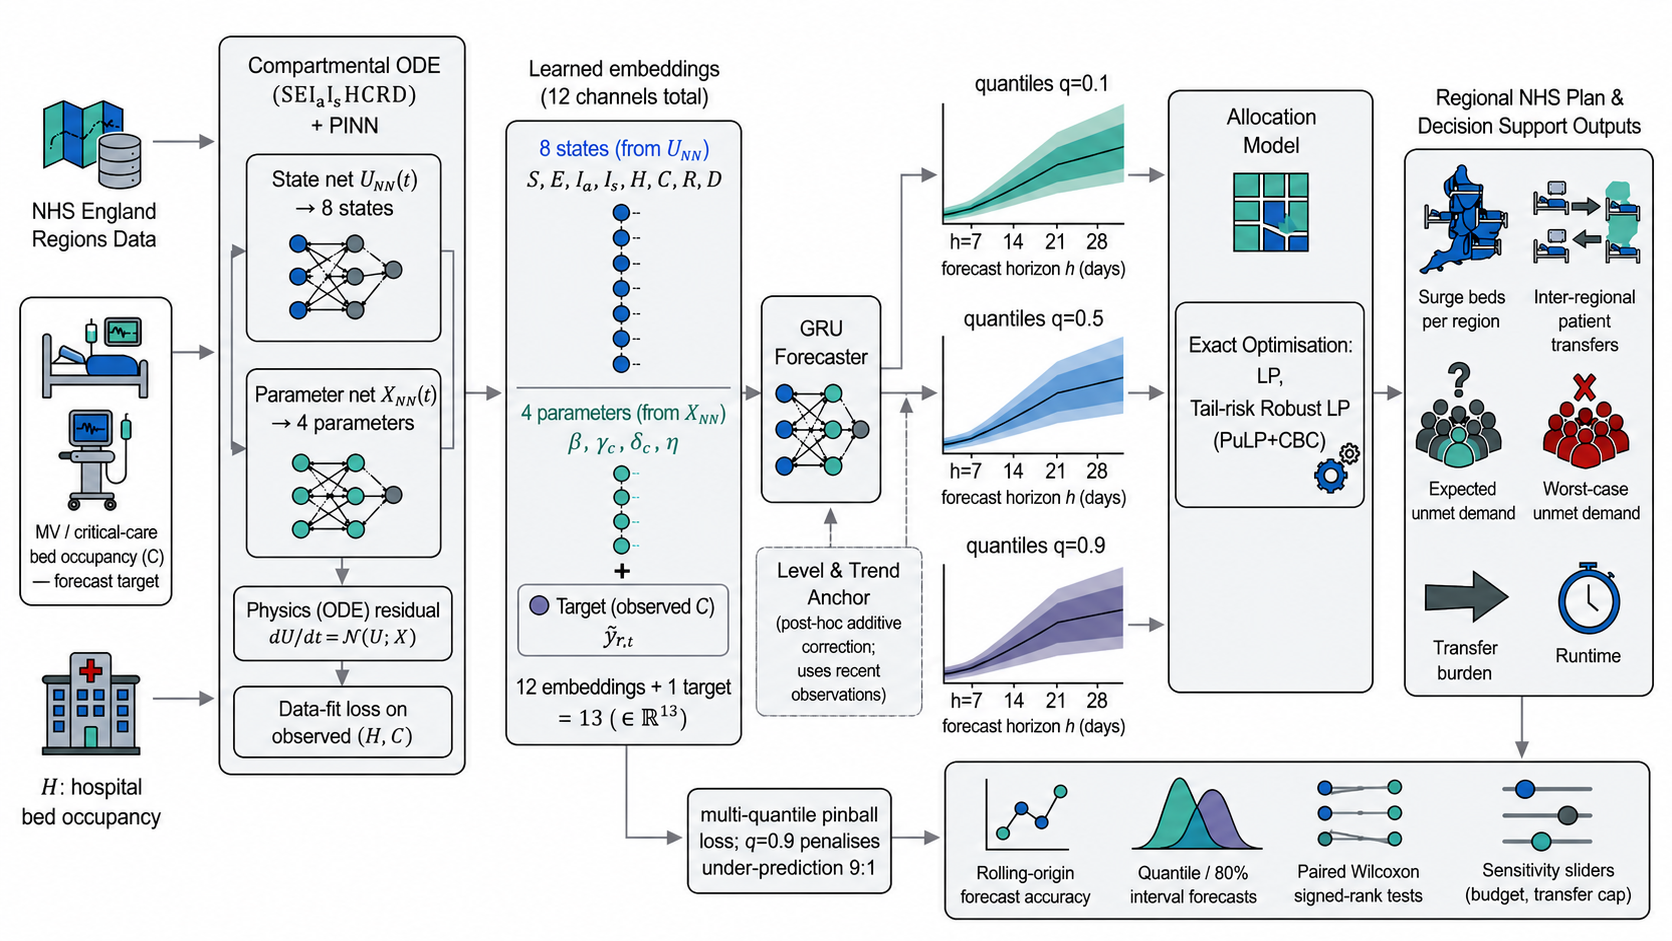
\includegraphics[width=\textwidth]{figure1.png}
\caption{Pipeline for NHS critical-care surge planning, from
regional data and physics-informed forecasting to scenario-based robust
allocation and evaluation.}
\label{fig:pipeline}
\end{figure*}

NHS critical-care surge planning during epidemic waves balances the
cost of pre-positioning capacity against the risk of unmet demand while
keeping inter-regional transfers manageable across the seven NHS England
regions. COVID-19 placed sustained pressure on adult
mechanical-ventilation capacity, making this a coupled forecasting and
allocation problem under regime shift. Existing forecasting work spans
statistical and recurrent baselines~\cite{ajao2024deep}, graph-based
epidemic and hospital-demand models~\cite{gao2021stan,gao2023hoist},
and physics-informed neural networks~\cite{raissi2019physics,ajao2025hybrid,qian2025physics};
interval and quantile evaluation is also standard in epidemic forecast
hubs~\cite{bracher2021evaluating}. The closest ICU-occupancy comparator,
a bidirectional LSTM with lagged mobility features and MC-dropout
intervals on Lazio data~\cite{valente2022forecasting}, like most such
work targets a single health system rather than multi-region planning.
These forecasters are usually
optimised for symmetric statistical accuracy, although critical-care
planning has an asymmetric error cost: under-prediction risks stranded
patients, whereas over-prediction wastes prepared capacity.

On the allocation side, robust facility-location and health-resource
models handle demand uncertainty with MILP, two-stage optimisation, and
metaheuristics~\cite{eriskin2022robust,wan2023two,shamseddin2025optimization,deb2002fast}.
Bertsimas et al.~\cite{bertsimas2022where} couple DELPHI dynamics to a
bilinear MIP for vaccination-site location, while Luo and
Stellato~\cite{luo2024equitable} embed neural-ODE compartmental dynamics
inside a McCormick-relaxed facility-location model. Our setting differs
from Smart Predict-then-Optimize~\cite{elmachtoub2022smart}. The
forecaster is not trained through allocation regret, but its
multi-quantile pinball objective is cost-asymmetric and feeds a robust
optimisation layer. To our knowledge, no prior work combines
physics-informed forecasting of NHS regional critical-care demand with
cost-asymmetric quantile training and an exact robust linear-programming
allocation across the seven NHS England regions.

This paper presents a forecast-to-decision pipeline
(\Cref{fig:pipeline}) in four phases. \emph{Phase~A} pre-trains a
per-region PINN on the $SEI_aI_sHCRD$ ODE system; its twelve outputs
(eight compartmental states, four transmission and clinical parameters)
are frozen and passed to a temporal GRU head that emits the horizon-wise
quantiles $q^{(0.1)}$, $q^{(0.5)}$, $q^{(0.9)}$ under a multi-quantile
pinball loss whose $q^{(0.9)}$ branch penalises under-prediction
nine-to-one, with a level-and-trend anchor. \emph{Phase~B}
discretises these quantiles into three scenarios with weights
$\pi=(0.2,0.6,0.2)$. \emph{Phase~C} solves the allocation exactly as a
linear program (deterministic and tail-risk-robust) via PuLP$+$CBC
against three heuristic baselines on a shared LP-slave oracle.
\emph{Phase~D} reports operational metrics and a sensitivity analysis
over the forecaster, budget $B$, tail-risk weight $\lambda_3$, travel
cap $\tau$, and transfer cap $\kappa$.

The main contributions are as follows:
(1)~\textbf{Cost-asymmetric forecaster.} A multi-quantile pinball loss,
a level-and-trend anchor, and a leakage-free per-origin recalibration
reduce $h{=}14$ RMSE by $25\%$ relative to refitted ARIMA and $42\%$
relative to a per-region GRU, and make the model competitive across all
horizons (best at $h{=}7$--$21$ and level with refitted ARIMA at
$h{=}28$, where seasonal-naive leads).
(2)~\textbf{Robust LP allocation.} With unconstrained transfers the
hybrid-regional robust LP ties every budget-exhausting policy on
coverage and wins on transfer burden ($4.6\times$ below
population-proportional); constraining transfers (sparser network or
capped transfer service) breaks the tie, the proportional rules
concede up to $60\%$ more expected unmet demand, and the robust LP is
never beaten on coverage.

% =============================================================================
\section{Forecasting Module}\label{sec:forecasting}
% =============================================================================

\subsection{SEIRD Compartmental Model}\label{ssec:seird}

For each region $r \in \R$ with population $N_r$ we model the local
epidemic with an eight-compartment $SEI_aI_sHCRD$ system whose states
are the susceptible $S_r$, exposed $E_r$, asymptomatic and symptomatic
infectious $I_{a,r}$ and $I_{s,r}$, hospitalised $H_r$, critical-care
$C_r$, recovered $R_r$, and deceased $D_r$ populations of region $r$,
each a count of people and together summing to $N_r$. \Cref{fig:seird}
shows the flow topology, in which the distinct probabilities $\omega$
($I_s\!\to\!H$) and $\phi$ ($H\!\to\!C$) disambiguate the two clinical
thresholds. The system evolves as
\begin{equation}\label{eq:seird}
\begin{aligned}
\dot{S}_r     &= -\beta_r S_r (I_{s,r}+I_{a,r})/N_r + \eta_r R_r, \quad
\dot{E}_r      = \beta_r S_r (I_{s,r}+I_{a,r})/N_r - \alpha E_r, \\
\dot{I}_{s,r} &= \alpha\rho E_r - d_s I_{s,r}, \quad
\dot{I}_{a,r}  = \alpha(1-\rho)E_r - d_a I_{a,r}, \\
\dot{H}_r     &= d_s\omega I_{s,r} - (d_H + \mu) H_r, \quad
\dot{C}_r      = \phi\, d_H H_r - (\gamma_{c,r}+\delta_{c,r}) C_r, \\
\dot{R}_r     &= d_s(1{-}\omega)I_{s,r} + d_a I_{a,r}
                + (1{-}\phi)d_H H_r + \gamma_{c,r}C_r - \eta_r R_r, \\
\dot{D}_r     &= \mu H_r + \delta_{c,r} C_r,
\end{aligned}
\end{equation}
subject to the conservation constraint
$S_r + E_r + I_{a,r} + I_{s,r} + H_r + C_r + R_r + D_r = N_r$, where a
dot denotes a time derivative ($\dot S_r = \mathrm{d}S_r/\mathrm{d}t$).
The eight fixed clinical constants (values from~\cite{ajao2025hybrid},
Table~1) are the latent-to-infectious (incubation) rate $\alpha$, the
symptomatic fraction $\rho\in[0,1]$, the symptomatic and asymptomatic
infectious-removal rates $d_s$ and $d_a$, the hospital-outflow rate
$d_H$, the symptomatic hospitalisation probability $\omega\in[0,1]$
($I_s\!\to\!H$), the in-hospital mortality rate $\mu$ ($H\!\to\!D$), and
the critical-care escalation probability $\phi\in[0,1]$ ($H\!\to\!C$);
all rates have units of $\text{day}^{-1}$. The four time-varying,
region-specific parameters learned from data are the transmission rate
$\beta_r$, the critical-care recovery rate $\gamma_{c,r}$ ($C\!\to\!R$),
the critical-care death rate $\delta_{c,r}$ ($C\!\to\!D$), and the
immunity-waning rate $\eta_r$ ($R\!\to\!S$).

% Figure 2: SEIRD compartment graph
\begin{figure}[!hb]
\centering
\resizebox{0.96\columnwidth}{!}{%
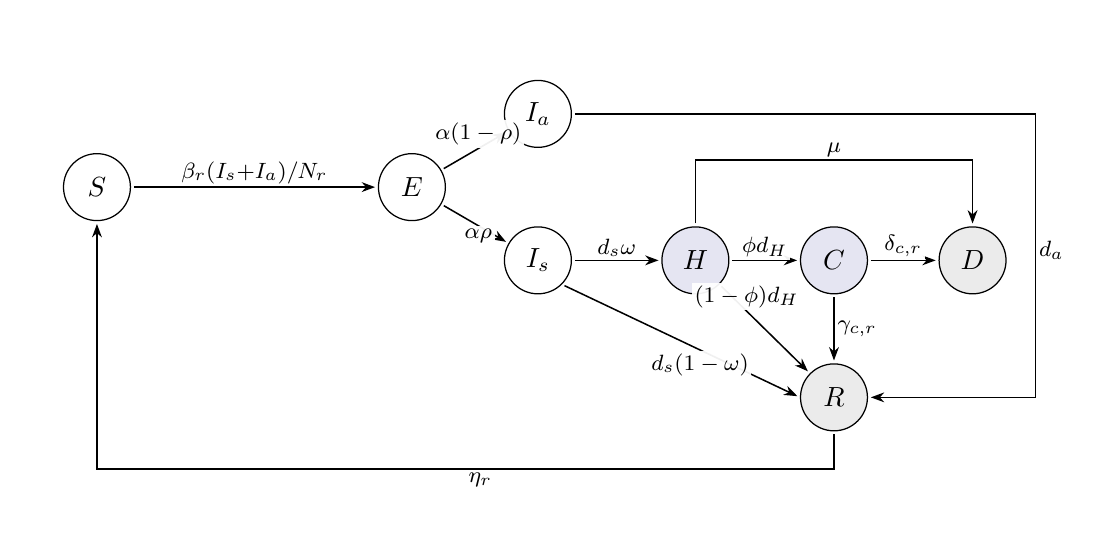
\begin{tikzpicture}[
  font=\small,
  >={Stealth[length=1.7mm,width=1.25mm]},
  x=16mm, y=15mm,
  comp/.style={draw, circle, minimum size=8.5mm, inner sep=0pt,
               line width=0.45pt, font=\normalsize\bfseries},
  observed/.style={fill=NavyBlue!10},
  terminal/.style={fill=black!8},
  edge/.style={->, line width=0.55pt, shorten >=1pt, shorten <=1pt},
  elabel/.style={font=\footnotesize, fill=white, inner sep=1pt,
                 fill opacity=0.94, text opacity=1},
]
\path[use as bounding box] (-2.05,-2.75) rectangle (6.25,1.35);
\node[comp]                       (S)  at (-1.5, 0) {$S$};
\node[comp]                       (E)  at (1, 0)    {$E$};
\node[comp]                       (Ia) at (2, 0.62) {$I_a$};
\node[comp]                       (Is) at (2,-0.62) {$I_s$};
\node[comp, observed]             (H)  at (3.25,-0.62) {$H$};
\node[comp, observed]             (C)  at (4.35,-0.62) {$C$};
\node[comp, terminal]             (D)  at (5.45,-0.62) {$D$};
\node[comp, terminal]             (R)  at (4.35,-1.78) {$R$};
\coordinate (Hdeath) at ($(H.north)+(0,0.56)$);
\coordinate (Ddeath) at ($(D.north)+(0,0.56)$);
\coordinate (IarecTop) at (5.95,0.62);
\coordinate (IarecDrop) at (5.95,-1.78);
\coordinate (Rwaning) at ($(R.south)+(0,-0.32)$);
\coordinate (Swaning) at ($(S.south)+(0,-2.10)$);

\draw[edge] (S) -- node[elabel, above] {$\beta_r(I_s{+}I_a)/N_r$} (E);
\draw[edge] (E) -- node[elabel, above, pos=0.55] {$\alpha(1-\rho)$} (Ia);
\draw[edge] (E) -- node[elabel, below, pos=0.55] {$\alpha\rho$} (Is);
\draw[edge] (Is) -- node[elabel, above] {$d_s\omega$} (H);
\draw[edge] (Is.south east) --
  node[elabel, below, pos=0.58] {$d_s(1-\omega)$} (R.west);
\draw[edge] (Ia.east) -- (IarecTop) --
  node[elabel, right, pos=0.48] {$d_a$} (IarecDrop) -- (R.east);
\draw[edge] (H) -- node[elabel, above] {$\phi d_H$} (C);
\draw[edge] (H.south east) --
  node[elabel, above, pos=0.30] {$(1-\phi)d_H$} (R.north west);
\draw[edge] (C) -- node[elabel, above] {$\delta_{c,r}$} (D);
\draw[edge] (C.south) --
  node[elabel, right, pos=0.50] {$\gamma_{c,r}$} (R.north);
\draw[edge] (H.north) -- (Hdeath) --
  node[elabel, above, pos=0.50] {$\mu$} (Ddeath) -- (D.north);
\draw[edge] (R.south) -- (Rwaning) --
  node[elabel, below, pos=0.48] {$\eta_r$} (Swaning) -- (S.south);
\end{tikzpicture}
}
\vspace{0.2ex}
\caption{$SEI_aI_sHCRD$ compartmental model used by the
physics-informed forecaster.}
\label{fig:seird}
\end{figure}

\subsection{Per-Region PINN-SEIRD}\label{ssec:pinn}

The PINN consists of two multilayer perceptrons (MLPs)
following~\cite{ajao2025hybrid}: a state
network $U^r_{NN}$ (five hidden layers of $20$ units) and a parameter
network $X^r_{NN}$ for $(\beta_r,\gamma_{c,r},\delta_{c,r},\eta_r)$
(three hidden layers of $20$ units), with tanh hidden activations and
sigmoid outputs. The loss combines a data fit on the two observable
compartments with an ODE residual against \Cref{eq:seird}. The observed
compartments are $H$ (daily general-and-acute hospital bed occupancy)
and $C$ (mechanical-ventilation [MV], i.e.\ critical-care, bed occupancy),
the only states with daily regional NHS counts; $C$ is the quantity the
temporal head forecasts and the allocation consumes as demand $\xi$:
\begin{equation}\label{eq:pinn_loss}
\begin{aligned}
\mathcal{L}^{PINN}_r
&= \sum_{t \in \T_{\text{train}}}\sum_{k \in \{H,C\}}
  \big(U^r_{NN,k}(t) - y_{r,t,k}/N_r\big)^2 \\
&\quad + \lambda_{ode}\sum_{t \in \T_{\text{coll}}}
  \Big\|\tfrac{dU^r_{NN}(t)}{dt} -
  \mathcal{N}(U^r_{NN}; X^r_{NN})\Big\|^2,
\end{aligned}
\end{equation}
where $\mathcal{N}$ is the right-hand side of \Cref{eq:seird},
derivatives use PyTorch autograd at $256$ collocation points sampled
uniformly in $\T_{\text{coll}}$, and observations are
population-normalised. We pre-train each region's PINN for $1500$ Adam steps with
$\lambda_{ode}=0.1$, $\text{lr}=5\!\times\!10^{-3}$; both terms converge
to the $2\text{--}8\times 10^{-6}$ range across regions.

With only $H$ and $C$ observed, the four learnable parameters
$(\beta_r, \gamma_{c,r}, \delta_{c,r}, \eta_r)$ are not jointly
identifiable ($\gamma_{c,r}$ and $\delta_{c,r}$ appear additively in
$\dot C_r$), so we make no per-trajectory interpretability claim: the
four-channel output is consumed as a learned feature vector by the GRU,
whose signal the ``w/o PINN params'' ablation confirms (\Cref{ssec:e1};
$h{=}14$ RMSE $14.46\!\to\!27.25$). Structural identifiability under
$\{H,C\}$ observation is future work.

\subsection{Temporal Head with Level-and-Trend Anchor}\label{ssec:temporal}

Once pre-trained the PINN is \emph{frozen}: at every origin, including
those in the Omicron test period, its networks are \emph{evaluated}
(never refit) to supply features, so any temporal extrapolation of the
state network beyond its Alpha/Delta fit is absorbed and corrected
downstream by the GRU and the anchor of \Cref{eq:anchor}. For each
lookback window of length
$L=28$ ending at origin $t$, the augmented feature sequence is
$\mathbf{f}_{r,i} = [U^r_{NN}(i)\,\|\,X^r_{NN}(i)\,\|\,
\tilde y_{r,i}] \in \mathbb{R}^{13}$, $i \in \{t-L+1,\dots,t\}$.
Here $U^r_{NN}(i)$ contributes all eight compartments (including the
never-observed latent $S,E,I_a,I_s,R,D$), so the head receives the full
physics-inferred state, and $\tilde y_{r,i}$ is the target z-scored with
training-period statistics only.
A two-layer
GRU (hidden $128$, dropout $0.15$) decodes the final hidden state via a
per-horizon two-layer MLP (width $64$, Gaussian-error-linear-unit
[GELU] activations) into standardised quantile
deltas $\Delta_{r,t}^{h,q}$ for $h\in\Hset=\{7,14,21,28\}$ and
$q\in\Qset=\{0.1,0.5,0.9\}$.

A \emph{level-and-trend anchor} makes the GRU's job residual:
\begin{equation}\label{eq:anchor}
\hat\zeta_{r,t}^{h,q} \;=\; \Delta_{r,t}^{h,q}
  \;+\; a^{h,q}\, \tilde y_{r,t}
  \;+\; g^{h,q}\, v_{r,t}^{(7)}\,
        \!\left(\tfrac{h}{7}\right)^{\!\!\psi^q},
\end{equation}
where $\tilde y_{r,t}$ is the most recent z-scored observation,
$v_{r,t}^{(7)} = \tilde y_{r,t}-\tilde y_{r,t-7}$ is the one-week slope,
and $a^{h,q},g^{h,q},\psi^q\in(0,1)$ are learnable scalars.
The Holt-Winters-style damping exponent $\psi^q$ prevents
slope-extrapolation overshoot at long horizons; we initialise
$\psi^{0.5}\!\approx\!0.88$ (near-linear) and
$\psi^{0.1}=\psi^{0.9}=0.5$ (square-root damping). Forecasts in
the original scale follow by inverting standardisation.

\subsection{Pinball Loss for Cost-Asymmetric Quantiles}\label{ssec:loss}

The forecaster minimises the multi-quantile pinball
loss~\cite{koenker1978regression}:
\begin{equation}\label{eq:pinball}
\mathcal{L}_{\text{pinball}} = \frac{1}{|\Qset|}\sum_{q\in\Qset}
  \mathbb{E}_{(t,h)}\!\big[\max\!\big(
    q\, e,\, (q{-}1)\, e\big)\big],\quad
    e = \tilde y_{r,t+h-1} - \hat\zeta_{r,t}^{h,q},
\end{equation}
evaluated at all $(h,q)\in\Hset\!\times\!\Qset$. The $q=0.5$ pinball
collapses to L1 (point accuracy); the $q=0.9$ pinball penalises
under-prediction nine-to-one. Splitting the kernel into its two arms,
$\max(q e,(q{-}1)e)=q\max(e,0)+(1{-}q)\max(-e,0)$, exposes it as a
convex newsvendor surrogate of the allocation's positive-part shortage
cost, with the $q{=}0.9$ asymmetry encoding that an under-bed risks a
stranded patient whereas an over-bed only wastes pre-positioned
capacity~\cite{elmachtoub2022smart}. The
forecaster is not trained through the allocation solver. We report $\hat y^{0.5}$
as the point forecast and $[\hat y^{0.1},\hat y^{0.9}]$ as an $80\%$
interval.

We train for up to $800$ AdamW epochs ($\text{lr}=10^{-3}$, weight decay
$10^{-4}$, cosine annealing) on one-day-stride Alpha-wave lookback
windows ($270$ per region, $1{,}890$ in total), with early stopping
(patience $80$) on the $1{,}134$ Delta-wave validation windows' pinball
loss. Once
selected, the model is frozen and applied to the Omicron test period via
$\Delta t = 7$-day rolling origins, yielding $32$ origin dates.

\subsection{Per-Origin Recalibration}\label{ssec:recal}
Applied frozen across a regime shift (high-demand Alpha/Delta training,
mild Omicron test), the point forecast inherits a systematic
over-prediction that grows with horizon. We correct it with two
steps. The first recalibrates the bias, subtracting at
each rolling origin $t$ and horizon $h$ the mean of the model's last
$K{=}3$ $h$-step errors whose target date is already observed ($<t$),
the adaptation that a per-origin refit gives for free. The second blends
with persistence, mixing the recalibrated forecast with
seasonal-naive($7$) under a per-horizon weight
$\alpha\in\{0,0.1,\dots,1\}$ fitted on an expanding window of realised
origins (pure model, $\alpha{=}1$, until seven origin--region pairs are
realised), so long horizons lean on persistence. Both use only
information available at $t$; the $80\%$ interval is left as the
quantile heads produce it, so the downstream allocation is unchanged.

% =============================================================================
\section{Regional Allocation Model}\label{sec:optimisation}
% =============================================================================

The allocation module decides how many surge beds to place in each NHS
region and how to route excess demand through inter-regional patient
transfers, given the quantile forecasts of \Cref{sec:forecasting}. We
present a deterministic linear program, a risk-averse (tail-weighted) extension,
and closed-form heuristic baselines.

\subsection{Sets, Parameters, and Decision Variables}\label{ssec:notation}

The scope is \emph{hybrid regional}, with demand nodes and capacity sites
coinciding with the seven NHS England commissioning regions, one set
$\R=\{r_1,\ldots,r_7\}$. Unlike facility-location models that choose
which sites to open~\cite{bertsimas2022where}, every region already
operates critical care, so there is no opening decision and surge cost
is uniform per bed; the model decides only bed counts and routing. The indices are regions $r,r'\!\in\!\R$; horizons
$h\!\in\!\Hset=\{7,14,21,28\}$~days; scenarios
$s\!\in\!\Sset=\{\text{low},\text{median},\text{high}\}$ from
$q^{(0.1)},q^{(0.5)},q^{(0.9)}$ with weights
$\pi=(0.2,0.6,0.2)$, a representative-quantile discretisation of lower,
central, and upper demand stress (a scenario mixture, not calibrated
probability bins).
The parameters are forecast demand
$\xi_{r,h}^s=\hat q_r^{(s)}(t_0+h)$; baseline critical-care capacity
$\Gamma_r=1.05\times$Delta-peak;
per-region surge cap
$K_r=0.5\,\Gamma_r$; budget
$B=0.20\sum_r \Gamma_r$; great-circle inter-centroid distance $\ell_{r r'}$ in
km ($\times 1.3$ road-detour); travel time
$T_{r r'}=60\,\ell_{r r'}/80$~min; mutual-aid cap $\tau=240$~min; outbound transfer cap $\kappa$
(uncapped at the headline operating point).
Decision variables fall in two layers. The \emph{first-stage} capacity
decision, the planner's only true control, is the surge allocation
$b_{r}\!\in\![0,K_r]$, shared across scenarios and horizons. The
per-scenario \emph{second-stage} recourse is the flow
$z_{r r',h}^s\!\geq\!0$ (defined for $T_{r r'}\!\leq\!\tau$); its
self-loop $z_{r r,h}^s$ is demand served \emph{locally} and its
off-diagonal ($r'\!\neq\!r$) entries are inter-regional transfers, with
unmet demand $u_{r,h}^s\!\geq\!0$ and a tail auxiliary $W\!\geq\!0$ for
the risk-averse variant. Of the $42$ ordered region pairs, $24$ satisfy
$T_{r r'}\!\leq\!\tau$ ($12$ undirected mutual-aid links); Midlands
reaches every region and South West only Midlands.

\subsection{Deterministic Median-Scenario LP}\label{ssec:milp}

For the median scenario $m$ ($q^{(0.5)}$), the deterministic model solves
\begin{equation}\label{eq:deterministic_objective}
\min\;
\textstyle\sum_{r,h} u_{r,h}^{m}
\;+\;\theta\sum_{r\neq r',h} \ell_{r r'}\, z_{r r',h}^{m},
\end{equation}
with $\theta=10^{-3}$ a transfer tie-break weight (one bed of weekly
snapshot unmet outweighs $1000$~patient-km of transfer). The objective
minimises \emph{unmet demand}; the second term only breaks ties between
equal-coverage plans by preferring less patient transport, so the surge
beds $b$ are placed to reduce shortage, not to minimise transfers. Each
$u_{r,h}^{m}$ is a snapshot of bed-shortfall at the weekly checkpoint
$h$, so the objective is the snapshot unmet summed over the four-week
planning horizon, not a continuous bed-day integral. The model is subject to
\begin{align}
z_{r r,h}^{m}+\!\!\textstyle\sum_{r'\neq r:\,T_{r r'}\leq\tau}\! z_{r r',h}^{m} + u_{r,h}^{m}
  &= \xi_{r,h}^{m}
  && \forall r,h, \label{eq:demand}\\
z_{r r,h}^{m}+\!\!\textstyle\sum_{r'\neq r:\,T_{r' r}\leq\tau}\! z_{r' r,h}^{m}
  &\leq \Gamma_r + b_{r}
  && \forall r,h, \label{eq:capacity}\\
\textstyle\sum_{r'\neq r}\, z_{r r',h}^{m} &\leq \kappa
  && \forall r,h, \label{eq:transfercap}\\
\textstyle\sum_r b_r &\leq B,
  && \label{eq:budget}\\
z_{r r',h}^{m} &= 0
  && \text{if } T_{r r'}\!>\!\tau, \label{eq:travel}\\
b_{r},z_{r r',h}^{m},u_{r,h}^{m} &\geq 0.
\end{align}
\Cref{eq:demand} is a demand balance. Each region's forecast demand is
served locally ($z_{r r,h}^{m}$), transferred to a reachable region
($z_{r r',h}^{m}$, $r'\!\neq\!r$), or left unmet ($u_{r,h}^{m}$).
\Cref{eq:capacity} caps the beds a region uses (local plus
transferred-in patients) at baseline plus surge; \Cref{eq:transfercap}
bounds outbound patients by the transfer-service capacity $\kappa$;
\Cref{eq:budget} charges the budget once per region; \Cref{eq:travel}
suppresses transfers beyond the mutual-aid window. As $u_{r,h}^{m}$ is
minimised, \Cref{eq:demand} holds it at the residual shortfall
$\max(0,\, \xi_{r,h}^{m}-\sum_{r'} z_{r r',h}^{m})$, a derived quantity
rather than a free decision.

\subsection{Risk-Averse Tail-Weighted Objective}\label{ssec:robust}

To hedge against the high-demand scenario the risk-averse model imposes
\Cref{eq:demand,eq:capacity,eq:transfercap} for every $s\in\Sset$,
retains \Cref{eq:budget,eq:travel}, and adds a tail term $\lambda_3 W$
($W\geq\sum_{r,h} u_{r,h}^s$ for $s\in\Sset_{\text{tail}}=\{\text{high}\}$),
giving the objective
\begin{equation}\label{eq:robust_objective}
\min\;
\sum_{s\in\Sset}\!\pi_s\!\Big(
\textstyle\sum_{r,h} u_{r,h}^s + \theta \sum_{r\neq r',h} \ell_{r r'} z_{r r',h}^s
\Big)\;+\;\lambda_3\, W.
\end{equation}
This is a \emph{scenario-weighted} LP that up-weights the high-demand
tail, not robust optimisation in the formal sense. With a single tail
scenario, minimisation drives $W=\sum_{r,h}u_{r,h}^{\text{high}}$, so
$\lambda_3 W$ is a linear penalty on the worst-scenario shortfall
(equivalently, extra weight on the high scenario) rather than a
Rockafellar--Uryasev conditional value-at-risk (CVaR); the auxiliary
form generalises unchanged to multiple tail scenarios. We call it the
\emph{robust LP} for brevity and report $\lambda_3{=}1$ throughout
($\lambda_3{=}0$ recovers the risk-neutral objective and
$\lambda_3\!\to\!\infty$ a worst-case policy on the high scenario); the
tail term binds only under tight budgets (\Cref{ssec:e5_e6}). Imposing
$q^{(0.9)}$ jointly across regions and horizons makes the construction
co-monotone, its tail over-conservative relative to the true joint
distribution; we treat this as an explicit stress-test choice and
examine its efficiency cost in \Cref{ssec:e5_e6}.

\subsection{Exact LP Solution and Baselines}\label{ssec:solvers}

Both models are linear programs ($7$ surge variables, $84$ self-loops,
up to $504$ transfer flows, $84$ unmet variables, and the tail
auxiliary, all continuous); a deployed plan rounds the per-region surge
to integers, changing total coverage by at most a few beds at this
budget. We solve them exactly in PuLP with the bundled COIN-OR
Branch-and-Cut (CBC) solver; at seven-region scale each instance reaches
global optimality in $<\!0.1$~s, so metaheuristic search is deferred to
the trust-level extension (\Cref{sec:conclusion}).

Every policy is scored on equal footing by a common LP re-evaluation.
For a fixed surge $\mathbf{b}^\star$ ($\sum_r b^\star_r\leq B$,
$b^\star_r\leq K_r$), the residual problem in $(z,u)$ fills in transfers
and unmet demand across all three scenarios, giving honest $E[u]$ and
$u^{\text{worst}}$ for the deterministic, robust, and heuristic
allocations alike.

Finally, three closed-form heuristics give a no-optimisation floor.
Population-proportional uses ONS region populations,
demand-proportional uses expected peak demand, and greedy
shortage-first adds single-bed increments to the most-unmet
region. Each fixes $\mathbf{b}^\star$, completed by the same LP step.

% =============================================================================
\section{NHS England Case Study}\label{sec:case_study}
% =============================================================================

The case study uses two public sources covering $1$~Aug~$2020$ -- $31$~Aug~$2022$ (the period of daily NHS regional publication). These are NHS~England COVID-19~Hospital~Activity~\cite{nhs_covid_activity}, which provides daily hospital and mechanical-ventilation bed occupancy at NHS regional resolution; and ONS Mid-Year Population Estimates~\cite{ons_mye_2021} on 2021 geography, used as the per-region PINN normaliser and the population-proportional baseline denominator. All experiments use the seven NHS England commissioning regions. The series is split chronologically by epidemic wave, so the most clinically distinct wave is held out, with training on $1$~Aug~$2020$ -- $31$~May~$2021$ (Alpha and early vaccination), validation on $1$~Jun~$30$ -- $2021$~Nov~$2021$ (Delta) for hyper-parameter selection and
early stopping, and testing on $1$~Dec~$2021$ -- $31$~Aug~$2022$ (Omicron and post-Omicron). Omicron's case-to-hospitalisation and
hospitalisation-to-critical-care ratios differ markedly from those of earlier waves, providing a regime-shift stress test.

For the allocation problem, baseline capacity $\Gamma_r$ is \emph{measured}
as each region's Delta-wave peak MV-bed occupancy $\times 1.05$, whereas
the per-region surge cap $K_r=0.5\,\Gamma_r$, total budget
$B=0.20\sum_r \Gamma_r\approx213$~beds (the surge headroom above the
$\sum_r\Gamma_r\approx1065$-bed measured baseline, not existing beds),
mutual-aid travel cap $\tau=240$~min, and
uncapped outbound transfers ($\kappa=\infty$) are
planning assumptions. The surge $b_r$ is the model's decision, with the
extra MV beds a region stands up above its measured baseline. The
forecaster, budget $B$, tail weight $\lambda_3$, travel cap $\tau$, and
transfer cap $\kappa$ are each swept in \Cref{ssec:e5_e6}. Forecast
metrics are macro-averaged across
the seven regions and the $32$ rolling-origin evaluations spanning the
Omicron test period; the full solver comparison is reported at the first
Omicron decision origin ($29$~Dec~$2021$), with an
all-origin check in \Cref{ssec:e5_e6}.
These are stress-test settings, not NHS standards: the $5\%$ uplift is
a headroom proxy, $K_r$ prevents unlimited concentration, and the
$20\%$ budget and $240$-min window form a generous headline case.
Deployment requires staffed-bed inventories, local expansion and
transfer limits, network travel times, and joint residuals for scenario
probabilities; our proxy supports policy comparison, not deployable
bed-count claims.

% =============================================================================
\section{Results and Discussion}\label{sec:results}
% =============================================================================

All results use the Omicron test split (1~Dec~2021--31~Aug~2022).

\subsection{Forecasting Accuracy}\label{ssec:e1}

\Cref{tab:forecast_accuracy} reports per-horizon RMSE and the
$h{=}28$ underestimation rate against four baselines under a common
$32$-origin rolling-origin protocol. The \emph{raw} PinnGRU point
forecast (frozen PINN encoder of \Cref{ssec:pinn} with the GRU head of
\Cref{ssec:temporal}) wins $h{=}7$ and $h{=}14$---paired origin-level
tests confirm the $h{=}14$ gain over ARIMA ($-3.88$ MV beds, Wilcoxon
$p{=}0.003$)---but degrades at long
horizons, where a regime-shift over-prediction bias (its $h{=}28$
underestimation rate is only $10.3\%$) leaves it behind ARIMA and
seasonal-naive ($+5.53$ MV beds vs ARIMA at $h{=}28$, $p{=}0.006$). A
leakage-free per-origin recalibration (\Cref{ssec:recal}) removes this
bias and blends with persistence at long horizons: the recalibrated
model is best at $h{=}7$, $14$ and $21$---cutting the operational
$14$-day RMSE by $25\%$ over ARIMA and $42\%$ over the per-region
GRU---and at $h{=}28$ ties ARIMA ($28.5$ vs $28.0$), with only
seasonal-naive ($26.0$) still ahead. Its $h{=}28$ underestimation rate
rises to $37\%$: the point forecast is now a well-calibrated median, not
a systematic over-predictor.

A second observation concerns the non-ARIMA models. XGBoost and the
per-region GRU are lag-only learners bounded by the $28$-day window;
unable to extrapolate into Omicron's altered case-to-hospitalisation
regime, they degrade sharply ($h{=}28$ RMSE $58.9$ and $44.0$). ARIMA's
per-origin refit keeps its degradation modest, and the recalibrated
PinnGRU matches it across horizons, consistent with the ``w/o PINN
params'' ablation isolated next.

The bottom block of \Cref{tab:forecast_accuracy} ablates three
load-bearing components. Replacing the pinball loss with MSE inflates
$h{=}14$ RMSE by $29\%$; zeroing the four PINN parameter features
inflates it almost two-fold ($14.46\!\to\!27.25$, the largest regression
in the table); and skipping PINN pre-training inflates it by $19\%$
($\to\!17.27$), confirming that the physics prior, not capacity, drives
the gain over the per-region GRU.

\begin{table}[t]
\caption{Forecast accuracy and ablations, macro-averaged over seven
NHS regions and $32$ rolling origins. \textbf{Bold}: best;
\underline{underline}: second best, per column (among the baselines and
the proposed model). MASE is the horizon-averaged mean absolute scaled
error (scaled by the in-sample seasonal-naive($7$) MAE; $<\!1$ beats
that benchmark, lower is better).}
\label{tab:forecast_accuracy}
\centering
\renewcommand{\arraystretch}{1.02}
\setlength{\tabcolsep}{4pt}
\begin{tabular}{lcccc@{\hskip 1em}c}
\toprule
\textbf{Model} & \multicolumn{4}{c}{\textbf{RMSE by horizon (days)}}
               & \textbf{MASE} \\
\cmidrule(lr){2-5}
               & 7 & 14 & 21 & 28 & \textbf{(all $h$)} \\
\midrule
Seasonal-naive(7)             & 13.53 & 18.16 & \underline{22.31} & \textbf{25.98} & 0.63 \\
ARIMA per region              & 11.33 & 17.80 & 23.41 & \underline{28.02} & \underline{0.61} \\
XGBoost (lag features)        & 12.45 & 22.90 & 36.42 & 58.88 & 0.89 \\
GRU per region                & 14.13 & 22.92 & 33.35 & 43.97 & 0.90 \\
PinnGRU (raw)                 & \underline{11.02} & \underline{14.46} & 24.19 & 34.63 & 0.77 \\
\textbf{PinnGRU+recal (prop.)} & \textbf{10.56} & \textbf{13.34} & \textbf{20.79} & 28.54 & \textbf{0.56} \\
\midrule
\quad w/o cost-asymmetric loss & 14.79 & 18.70 & 27.09 & 41.47 & 0.97 \\
\quad w/o PINN pre-training   & 12.26 & 17.27 & 22.56 & 34.73 & 0.76 \\
\quad w/o PINN params         & 23.97 & 27.25 & 32.94 & 44.59 & 1.23 \\
\bottomrule
\end{tabular}
\end{table}

\subsection{Allocation Performance Across Solvers}
\label{ssec:e2_e3}

\Cref{tab:allocation} compares the allocation policies on the
seven-region problem with $B = 213$~beds ($20\%$ of total baseline), four-hour
mutual-aid cap, and PinnGRU $q^{(0.1)}\!/q^{(0.5)}\!/q^{(0.9)}$
forecasts at the first Omicron-period origin. Every policy's chosen
allocation is re-scored by the common LP re-evaluation over the full
three-scenario set so $E[u]$ and $u^{\text{worst}}$ are reported on
equal footing.

\textbf{(i)} The \emph{robust LP} achieves the lowest transfer
burden in the table ($672$~bed-km, $4.6\times$ below
population-proportional and $1.7\times$ below greedy shortage-first),
but this is a tie-break among policies with identical rounded $E[u]$
and $u^{\text{worst}}$, not a coverage improvement. \textbf{(ii)} The
\emph{deterministic LP} spends only $51$ of the $213$ available beds
and pays $\sim\!3\times$ higher $E[u]$ and $u^{\text{worst}}$,
quantifying the value of $\pi_s$-weighted expectation over median-only
optimisation. \textbf{(iii)} The robust LP therefore wins on
\emph{routing} rather than coverage. Once the budget binds, every
budget-exhausting policy ties on $E[u]$ and $u^{\text{worst}}$ and
differs only on transfer burden.

\begin{table}[t]
\caption{Allocation comparison under $B = 213$~beds, $\tau = 240$~min,
and three PinnGRU scenarios.}
\label{tab:allocation}
\centering
\renewcommand{\arraystretch}{1.02}
\setlength{\tabcolsep}{4pt}
\begin{tabular}{lrrrrr}
\toprule
\textbf{Policy} & \textbf{Beds} & \textbf{$E[u]$}
                & \textbf{$u^{\mathrm{worst}}$} & \textbf{Transfer}
                & \textbf{Time}\\
                & & & & \textbf{(bed\,km)} & \textbf{(s)}\\
\midrule
Population-proportional    & 212.7 & 29.0  & 144.8 & 3119.8  & 0.00 \\
Demand-proportional        & 212.7 & 29.0  & 144.8 & 2615.3  & 0.00 \\
Greedy shortage-first      & 212.7 & 29.0  & 144.8 & 1140.0  & 9.98 \\
Deterministic LP           &  51.4 & 83.3  & 416.4 & 1175.1  & 0.03 \\
\textbf{Robust LP ($\lambda_3{=}1$)}
                           & 212.7 & 29.0  & 144.8 & \textbf{671.7} & 0.04 \\
\bottomrule
\end{tabular}
\end{table}

Inspecting the regional structure behind \Cref{tab:allocation}
(\Cref{fig:alloc_budget}a), the deterministic LP surges only Midlands
and South East (where median demand exceeds baseline); budget-exhausting
policies all cover those two and differ on the rest, the robust LP
finding a compromise with non-trivial North~West and London surge.

\begin{figure}[ht]
\centering

\includegraphics[width=\textwidth]{fig_alloc_budget.png}
\caption{(a)~Per-region peak surge allocation (beds) by policy at the
first Omicron origin. (b)~Exact robust-LP cost--shortage frontier
showing how expected and worst-case unmet demand fall as the surge
budget $B/\sum_r C_r$ grows. This is the decision-relevant trade-off a
planner navigates.}
\label{fig:alloc_budget}
\end{figure}

\subsection{Forecast-Quality and Parameter Sensitivity}
\label{ssec:e5_e6}

\paragraph{Forecast-quality robustness.}
Substituting each forecaster into the robust LP at the $29$~Dec~$2021$
origin, the $q^{(0.9)}$ peak sums (PinnGRU $1421$, XGBoost $1105$, GRU
$973$, ARIMA $875$, seasonal-naive $745$~beds) all exceed the realised
peak ($797$) except seasonal-naive. Realised unmet is zero throughout,
including the oracle, so this origin cannot separate policies on
realised coverage: forecast quality buys \emph{efficiency} at the
$q^{(0.9)}$ margin, not coverage, in this mild Omicron instance.

Across all $32$ Omicron origins the pattern holds: robust LP,
population-proportional, and demand-proportional allocations share a
mean expected unmet of $2.9$, but the robust LP cuts mean transfer
burden to $76$~bed-km versus $406$ and $337$~bed-km. The proportional
baselines fill the full $212.7$-bed budget at every origin, whereas the
robust LP scales surge to local demand (mean total surge $35.4$~beds,
hitting the cap only at peaks), so the routing-efficiency gain holds
across the full demand distribution.

\paragraph{Parameter sensitivity.}
A one-at-a-time sweep isolates each control. The budget $B$ dominates
(\Cref{fig:alloc_budget}b): $B/\sum_r C_r$ from $0.20$ to $0.10$ doubles
$E[u]$ and triples $u^{\text{worst}}$, while $0.30$ cuts $E[u]$ to
$\sim\!1/4$. $\lambda_3$ is \emph{non-binding} at $B=0.20$ (the
expectation-minimising solution already clears the high tail); only a
tighter budget ($\leq\!15\%$) re-engages it. The travel cap
$\tau\!=\!120$~min cuts transfer burden by $34\%$ at a $3\%$ rise in
$E[u]$; $\tau\!\geq\!240$~min is slack.

% Table 3 (one-at-a-time sensitivity sweep) removed for the 12-page UKCI
% limit: the budget/tail-penalty/travel-cap effects are reported in the prose
% above and the exact budget frontier is Fig.~4(b). The full sweep CSVs
% (e6_*.csv) remain in the repository for the journal extension.

% =============================================================================
\section{Conclusion}\label{sec:conclusion}
% =============================================================================

We presented a forecast-to-decision pipeline for NHS critical-care
surge planning that couples a per-region physics-informed forecaster to
a tail-risk robust allocation linear program. With a leakage-free
per-origin recalibration, PinnGRU is competitive across the horizons
that drive surge decisions, cutting $14$-day RMSE by $25\%$ over
re-fitted ARIMA and $42\%$ over a neural GRU. On the decision side the
gain is structural: once the budget binds, every budget-exhausting
policy ties on coverage and the robust formulation wins by routing the
same surge with the least patient transfer. Principal caveats are
detour-scaled travel times, well-mixed populations, scaled cost units,
and a single realised origin. A deeper limitation couples the modules:
the per-region forecaster and co-monotone scenarios over-state the joint
tail and understate transfers, which pay off most under
\emph{asynchronous} regional peaks. Correlated demand scenarios from the
joint forecast distribution, and a trust-level instance where exact
solution grows expensive enough to warrant metaheuristics, are the
natural next steps.


% =============================================================================
% \section*{Conflict of Interest}
% Vasile Palade is Conference Co-Chair of UKCI~2026. This is declared
% in the submission record and the paper's review allocation was handled
% accordingly.

% Bibliography
% Springer Math/Physics/Computer Science BibTeX style from the SVProc bundle.
\bibliographystyle{spmpsci}
\bibliography{references}

\end{document}
